
% !TeX document-id = {a90a2b0a-e08e-44ed-850a-35793bedbf3a}
% !TeX TS-program = xelatex

% !BIB program = biber
\documentclass[handout]{beamer}
%\documentclass[compress]{beamer}
\usepackage[T1]{fontenc}
\usepackage{pifont}
\usetheme[block=fill,subsectionpage=progressbar,sectionpage=progressbar]{metropolis} 


\definecolor{Purple}{HTML}{911146}
\definecolor{Orange}{HTML}{CF4A30}

% Theme colors are derived from these two elements
\setbeamercolor{alerted text}{fg=Orange}

% ... however you can of course override styles of all elements
\setbeamercolor{frametitle}{bg=Purple}


\usepackage{wasysym}
\usepackage{etoolbox}
\usepackage[utf8]{inputenc}

\usepackage{threeparttable}
\usepackage{subcaption}

\usepackage{tikz-qtree}
\setbeamercovered{still covered={\opaqueness<1->{5}},again covered={\opaqueness<1->{100}}}


\usepackage{listings}

\lstset{
	basicstyle=\scriptsize\ttfamily,
	columns=flexible,
	breaklines=true,
	numbers=left,
	%stepsize=1,
	numberstyle=\tiny,
	backgroundcolor=\color[rgb]{0.85,0.90,1}
}



\lstnewenvironment{lstlistingoutput}{\lstset{basicstyle=\footnotesize\ttfamily,
		columns=flexible,
		breaklines=true,
		numbers=left,
		%stepsize=1,
		numberstyle=\tiny,
		backgroundcolor=\color[rgb]{.7,.7,.7}}}{}


\lstnewenvironment{lstlistingoutputtiny}{\lstset{basicstyle=\tiny\ttfamily,
		columns=flexible,
		breaklines=true,
		numbers=left,
		%stepsize=1,
		numberstyle=\tiny,
		backgroundcolor=\color[rgb]{.7,.7,.7}}}{}


\usepackage[american]{babel}
\usepackage{csquotes}
\usepackage[style=apa, backend = biber]{biblatex}
\DeclareLanguageMapping{american}{american-UoN}
\addbibresource{../literature.bib}
\renewcommand*{\bibfont}{\tiny}

\usepackage{tikz}
\usetikzlibrary{shapes,arrows,matrix}
\usepackage{multicol}

\usepackage{subcaption}

\usepackage{booktabs}
\usepackage{graphicx}

\graphicspath{{../pictures/}}

\makeatletter
\setbeamertemplate{headline}{%
	\begin{beamercolorbox}[colsep=1.5pt]{upper separation line head}
	\end{beamercolorbox}
	\begin{beamercolorbox}{section in head/foot}
		\vskip2pt\insertnavigation{\paperwidth}\vskip2pt
	\end{beamercolorbox}%
	\begin{beamercolorbox}[colsep=1.5pt]{lower separation line head}
	\end{beamercolorbox}
}
\makeatother



\setbeamercolor{section in head/foot}{fg=normal text.bg, bg=structure.fg}



\newcommand{\question}[1]{
	\begin{frame}[plain]
		\begin{columns}
			\column{.3\textwidth}
			\makebox[\columnwidth]{
				
\includegraphics[width=\columnwidth,height=\paperheight,keepaspectratio]{../pictures/mannetje.png}}
			\column{.7\textwidth}
			\large
			\textcolor{orange}{\textbf{\emph{#1}}}
		\end{columns}
\end{frame}}

\newcommand{\instruction}[1]{\emph{\textcolor{gray}{[#1]}}}


\title[Computational Communication Science 2]{\textbf{Computational Communication Science 2} \\Week 7 - Lecture\\ »Rule-based vs. Automated Text Classification«}
\author[Marthe Möller, Anne Kroon]{Marthe Möller \\ Anne Kroon \\ ~ \\ \footnotesize{a.m.moller@uva.nl, @marthemoller \\a.c.kroon@uva.nl, @annekroon} \\}
\date{May, 2022}
\institute[Digital Society Minor, University of Amsterdam]{Digital Society Minor, University of Amsterdam}


\begin{document}
	
	\begin{frame}{}
		\titlepage
	\end{frame}
	
	\begin{frame}{Today}
		\tableofcontents
	\end{frame}
	
	
	\section{Rule-based Text Classification}
	
	\begin{frame}{Text Classification} 
		
	Text classification: To assign a label to a text.
	
	For example, to distinguish between:
	\begin{itemize}
		\item newspaper articles about sports vs. economics.
		\item reliable vs. unreliable information about vaccination.
		\item webpages about holding companies vs. financing companies.
		\item positive vs. negative movie reviews.
	\end{itemize}
	
	\end{frame}
		
	\begin{frame}{Studying Flaming (Example)} 
	
	RQ: How problematic is flaming on Twitter? \\
	Bag-of-words approach:
	
	\begin{enumerate}
		\item Create a list with all the swearwords that exist.
		\item For each tweet in the dataset, use the list to count the number of swearwords	
		\item If a tweet contains X number of swearwords label it as flaming
	\end{enumerate}
	

\end{frame}


	\begin{frame}{Sentiment Analysis} 
	
	We can add nuance by creating more rules.
	
	For example, in sentiment analyses, we can include a rule telling the machine what to do in case of negation or modifiers.
	
	"This movie is really not good." \\
	"This movie is really good."
		
	\end{frame}


	\begin{frame}{Rule-based Text Classifcation} 
	
	Advantages of rule-based text classification:
	\begin{itemize}
		\item Simple and therefore transparent
		\item Cheap
	\end{itemize}
	
	Challenges of rule-based text classification:
	\begin{itemize}
		\item Not a suitable way to anayze latent or abstract variables 
		\item You must know all the categories beforehand
		\item You must know and be able to express all the rules
	\end{itemize}

	\end{frame}


\begin{frame}{From Rule-based to Automated}

	When it is easy for humans to decide to what class a text belongs, but we struggle to translate our decision process into straight-forward rules, we are likely to be better of using a form of automated text classification: Supervised Machine Learning.
	
\end{frame}


	
	\section{SML}
	
	
	\begin{frame}{What is SML?}
		
		\begin{center}
			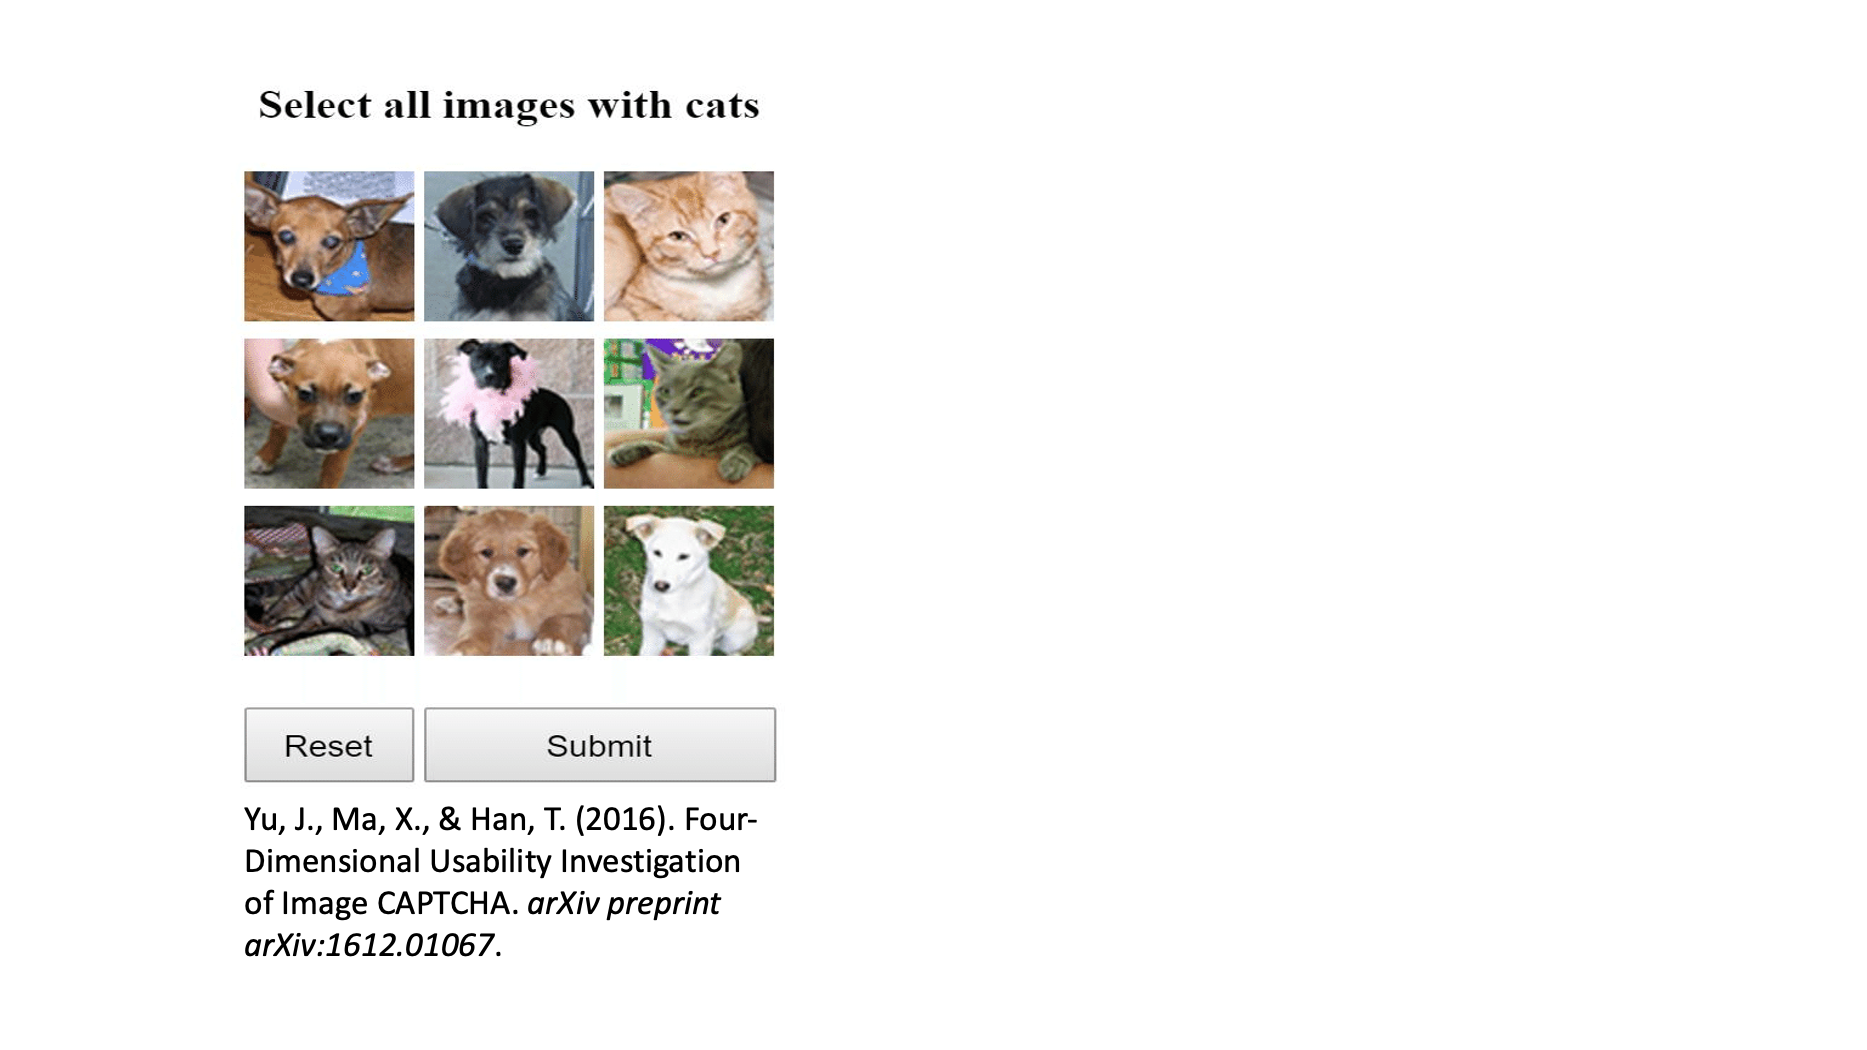
\includegraphics[width=4cm, height=7cm]{../pictures/CAPTCHA.png} 
		\end{center}
		
		
		% Probably all of you have come across an assignment like this one once when you tried to access a website. You asked to determine for each image if it depicts a cat. There are many variations to this assignment (e.g., select all the images with a traffic sign). The purpose of these assignments is to verify that a human is trying to enter a webpage as opposed to a machine. For this protection mechanism to work, it is assumed that while humans are able to distinguish pictures of cats from other pictures, machines cannot.
		
	\end{frame}
	
	
	\begin{frame}{What is SML?}
		
		\begin{center}
			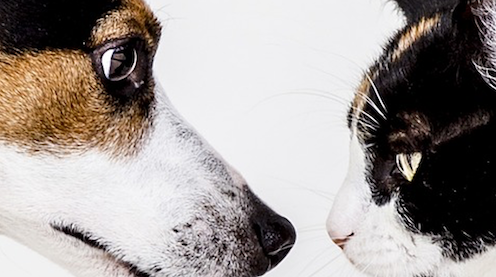
\includegraphics{../pictures/dogvscat.png}
		\end{center}
		
		\begin{tiny}
			Read more about this project in: 
			\fullcite{sermanet_overfeat_2014} 
		\end{tiny}
		
		
		% In 2013, Kaggle (Kaggle.com) challenged people to write a script teaching a computer to successfully complete the task of distinguishing images of cats from images of dogs.
		
		% To achieve their goal, contesters needed to use Machine Learning.
		
		% In this story, it is the process whereby the computer learns how to predict images’ score on a variable (let’s name it ‘animal’) which can be either (1) cat or (0) dog.
		
	\end{frame}
	
	\begin{frame}{What is SML?} 
		
		Supervised Machine Learning (SML): “A form of machine learning, where we aim to predict a variable that, for a least part of our data is known.” \\\
		
		\begin{tiny}
			\fullcite{van_atteveldt_computational_2022} 
		\end{tiny}
		
	
	\end{frame}
	
	
	\begin{frame}{What is SML?} 
		
		“The goal of Supervised Machine Learning: estimate a model based on some data, and then use the model to predict the expected outcome for some new cases, for which we do not know the outcome yet.” \\\
		
		\begin{tiny}
			\fullcite{van_atteveldt_computational_2022} 
		\end{tiny}
		
		
		
		% In this lecture, we focus on a specific type of machine learning, namely supervised machine learning.
		
		% In the cats-example, it would work as follows: We give the computer part of the images in a dataset, along with their scores on the animal-variable. Based on this part of the dataset, the computer “learns” which factors determine whether an image receives score 1 (cat) or score 0 (dog). The computer applies this to the remaining images (for which it was unknown whether they depicted a dog or a cat). So, the computer has ‘learned’ to distinguish cats from dogs. 
		
	\end{frame}
	
	\begin{frame}{What is SML?} 
		
		Machine Learning has a lot of similarities to regression analysis!
		
		% Communication scholars often use scores on some independent variables (for example: age, and gender) to calculate subjects’ scores on a dependent variable (for example: Instagram usage). They use a regression analysis to do this calculation.
		
	\end{frame}
	
	
	\section{The principles behind SML}
	
	\begin{frame}{The principles behind SML} 
		
		\(y = constant + b_1 * x_1 + b_2 * x_2\) 
		
		\(x_1\) = bark? (0= no, 1 = yes) \\\
		\(x_2\) = tail? (0 = no, 1 = yes) \\\
		\(y\) = Is this a dog? ( 0 = definitely no, 1 = definitely yes)
		
		% [Discuss the meaning of the formula, the constant and the regression coefficient]. By running the regression analysis, we retrieve values for the regression coefficients and the constant.
		
	\end{frame}
	
	
	\begin{frame}{The principles behind SML} 
		
		\(y = constant + b_1 * x_1 + b_2 * x_2\) \\\
		
		\(y = 0 + 0.8 * x_1 + 0.2 * x_2\) \\\
		
		
		% If we then fill out the scores of a participant on each independent variable, we can predict that person’s score on the dependent variable.
		
	\end{frame}
	
	\begin{frame}{The principles behind SML} 
		
		\(y = 0 + 08 * 1 + 0.2 * 0\) \\\
		
		\(0.8 = 0 + 0.8 * 1 + 0.2 * 0\) \\\
		
		% A computer could do this for an unlimited number of participants. So, say we have 1000 people. With the regression formula, we can predict for each person if they have an Instagram account or not based on their gender and age.
		
	\end{frame}
	
	\begin{frame}{The principles behind SML} 
		
		\(0.8 = 0 + 0.8 * 1 + 0.2 * 0\) \\\
		
		Classification: a predictive modeling problem where a class label is predicted for a given example of input data. 
		
		
		%(https://machinelearningmastery.com/types-of-classification-in-machine-learning/)
		
		% Note that while in more traditional research approaches, we focus on the value of the regression coefficient (e.g., the coefficient for education level or what is the effect of education on Instagram usage), in machine learning, we do not care so much about the exact regression coefficients. We merely use the coefficients to predict. 
		
		%These predicting tasks are known as classification. 
		
		
	\end{frame}
	
	
	\begin{frame}{The principles behind SML}
		
		\begin{center}
			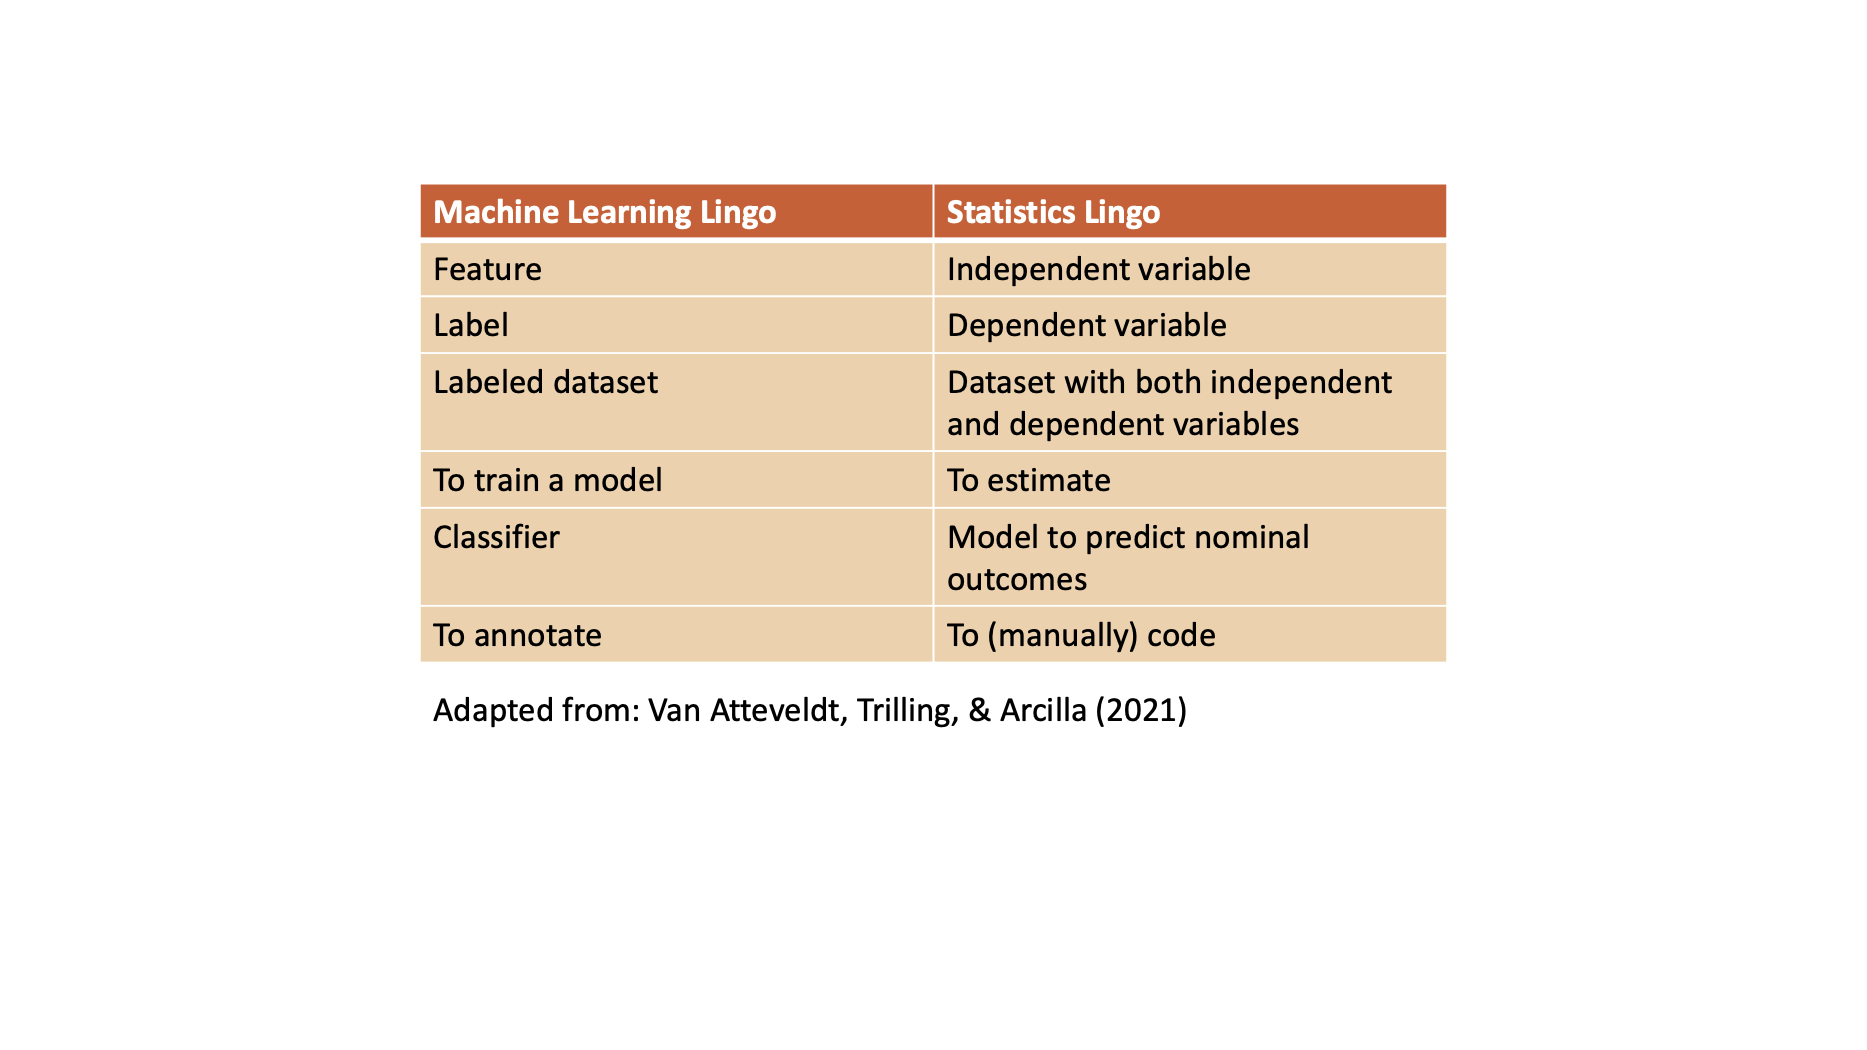
\includegraphics[width=\linewidth,height=\textheight,keepaspectratio]{../pictures/MLlingo.png} \\\
		\end{center}
		
		
		% Now that we are drawing comparisons between statistics and machine learning, let’s have a look at some machine learning lingo that you’ll bound to bump into.
		
	\end{frame}
	
	
	\begin{frame}{The principles behind SML} 
		
		Machine Learning: using a (regression) formula to predict a label. \\\
		
		Traditional usage of formulas in CS: to explain \\\
		
		Usage of formulas in ML: to predict \\\
		
		
		% ML is basically using something you already know to achieve a new goal.
		
		
	\end{frame}
	
	
	
	\begin{frame}{Zooming out} 
		
		We talked about:
		\begin{itemize}
			\item Rule-based Text Classification
			\item Automated Text Classification: SML
			\item The principles behind SML \\\
		\end{itemize}
		
		Next, we will talk about:
		\begin{itemize}
			\item Some commonly used SML models
		\end{itemize}
		
	\end{frame}
	
	
	\section{SML models}
	
	\begin{frame}{SML step by step}
		
		\begin{center}
			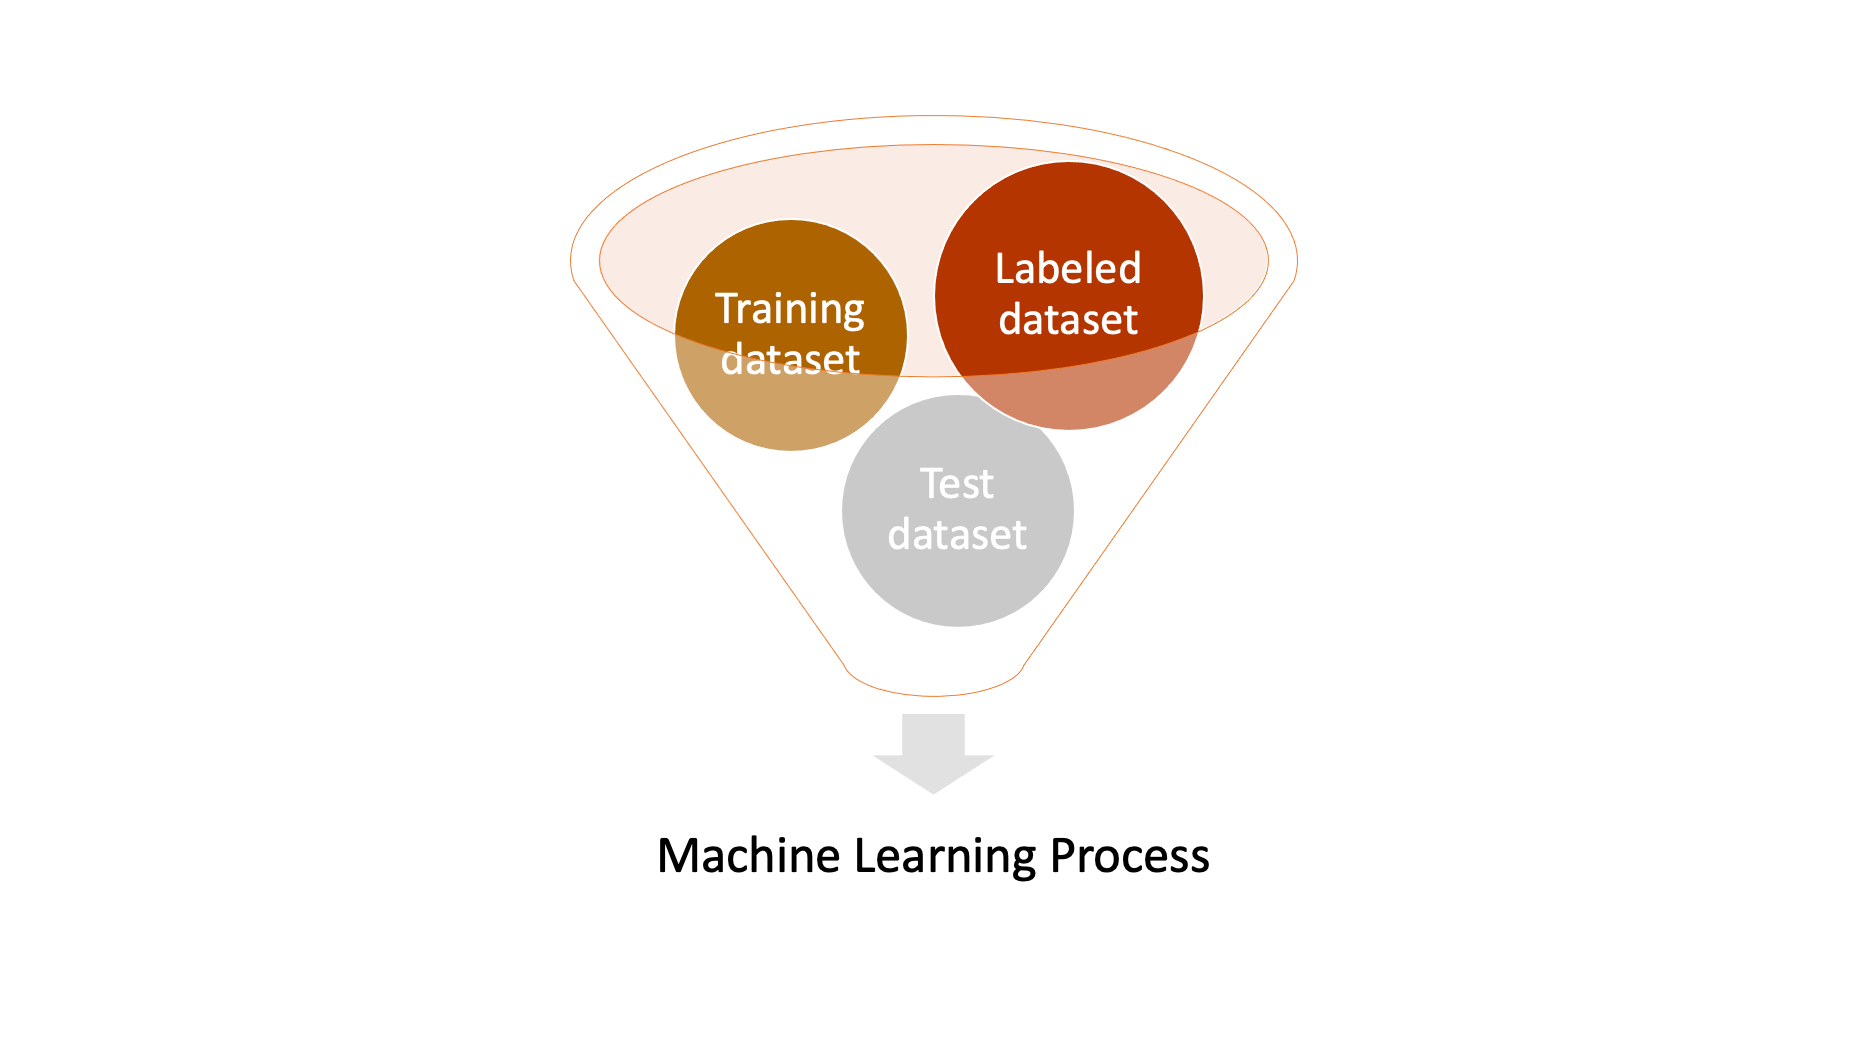
\includegraphics[width=\linewidth,height=\textheight,keepaspectratio]{../pictures/MLingredients.png} \\\
		\end{center}
		
		
		% To do SML, we need some ingredients. Namely, we need a labelled dataset. This is a dataset where for each case, the vales of the features (independent variables) and the labels (dependent variables) are known. We split this dataset into two parts. One part we call the training dataset and the other part we call the test dataset.
		
	\end{frame}
	
	
	\begin{frame}{SML step by step}
		
		\begin{center}
			
\includegraphics[width=\linewidth,height=\textheight,keepaspectratio]{../pictures/MLprocess.png} \\\
		\end{center}
	
		Let's have a look at some commonly used ML models.
		
		
		% With these ingredients, we can go through three steps.
		
		% First, we train our classifier, that is to say: We estimate our model using the training dataset.
		
		% If we connect this back to the regression equation we discussed earlier: We estimate the regression equation.
		
			% When we train a model, we can do so based on different functions. Any function can be used, as long as it uses features of cases as an input and produces a prediction based on these. 
		
		% Second, we test our classifier: We test how capable our model is to predict the correct labels. We do this using the test dataset.
		
		% (Why not use the same training dataset again? We could do this, but it would be a rather lenient test because the classifier has been trained on exactly these data. To truly assess how well our classifier performs, we need to use new data. We use the test data because for these data, we can verify if the classifier was correct (remember that the test data stems from our labeled dataset, so we know what the correct labels are!).
		
		% Third, we evaluate our classifier:
		% More about this later today and next week!
		
			% [note here the important assumption of SML: that the training set, test set, and the unlabeled data that are to be classified are (at least in principle and approximately) drawn from the same population. For example, you cannot train a classifier using movie reviews and then use that classifier to analyze Instagram comments]
		
		
	\end{frame}
	

\begin{frame}{Regression}
	
	\begin{center}
		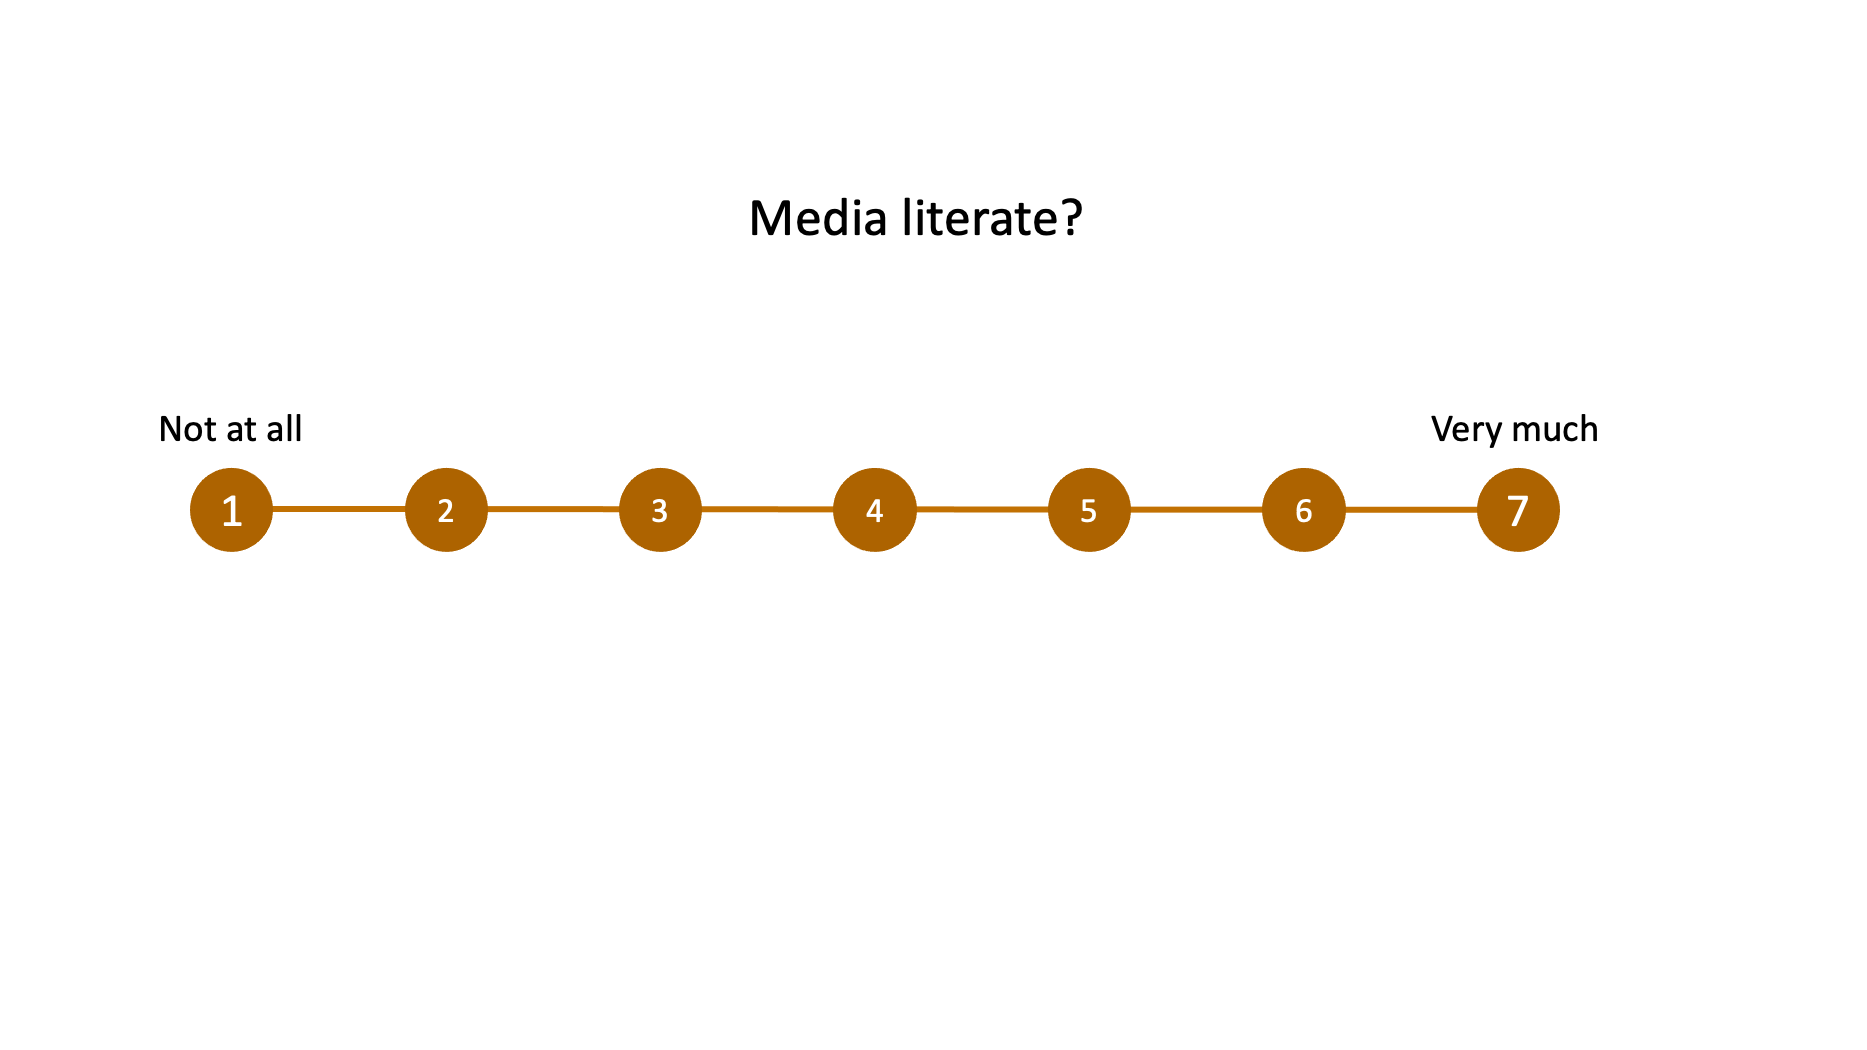
\includegraphics[width=\linewidth,height=\textheight,keepaspectratio]{../pictures/medialiteracyscale.png} \\\
	\end{center}
	
	
	% One model that can be used, is the ordinary least squares (OLS) regression model, like we just discussed.
	
	% You know from statistics courses that OLS regression predicts a case’s value on a dependent variable. For example, we use the scores of a case on two independent variables (say age and education level) to predict that persons score on a dependent variable: say, media literacy score ranging from 1 to 7.
	
	% Applying this to ML, we use the regression to predict the scores of many many cases on the DV. 
	
	
\end{frame}



\begin{frame}{Regression}
	
	\begin{center}
		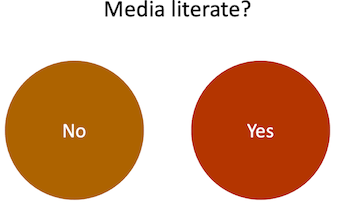
\includegraphics{../pictures/medialiteracydummy.png} \\\
	\end{center}
	
	
	% But in applications of ML, we are often not so much interested in predicting a specific value of the DV. Rather, we are interested in predicting categories. For example, based on some features, we want to predict if someone uses Instagram or not.
	
	% To predict nominal outcomes (such as Instagram user, yes or no), we use logistic regression.
	
	
\end{frame}


\begin{frame}{Regression}
	
	\begin{center}
		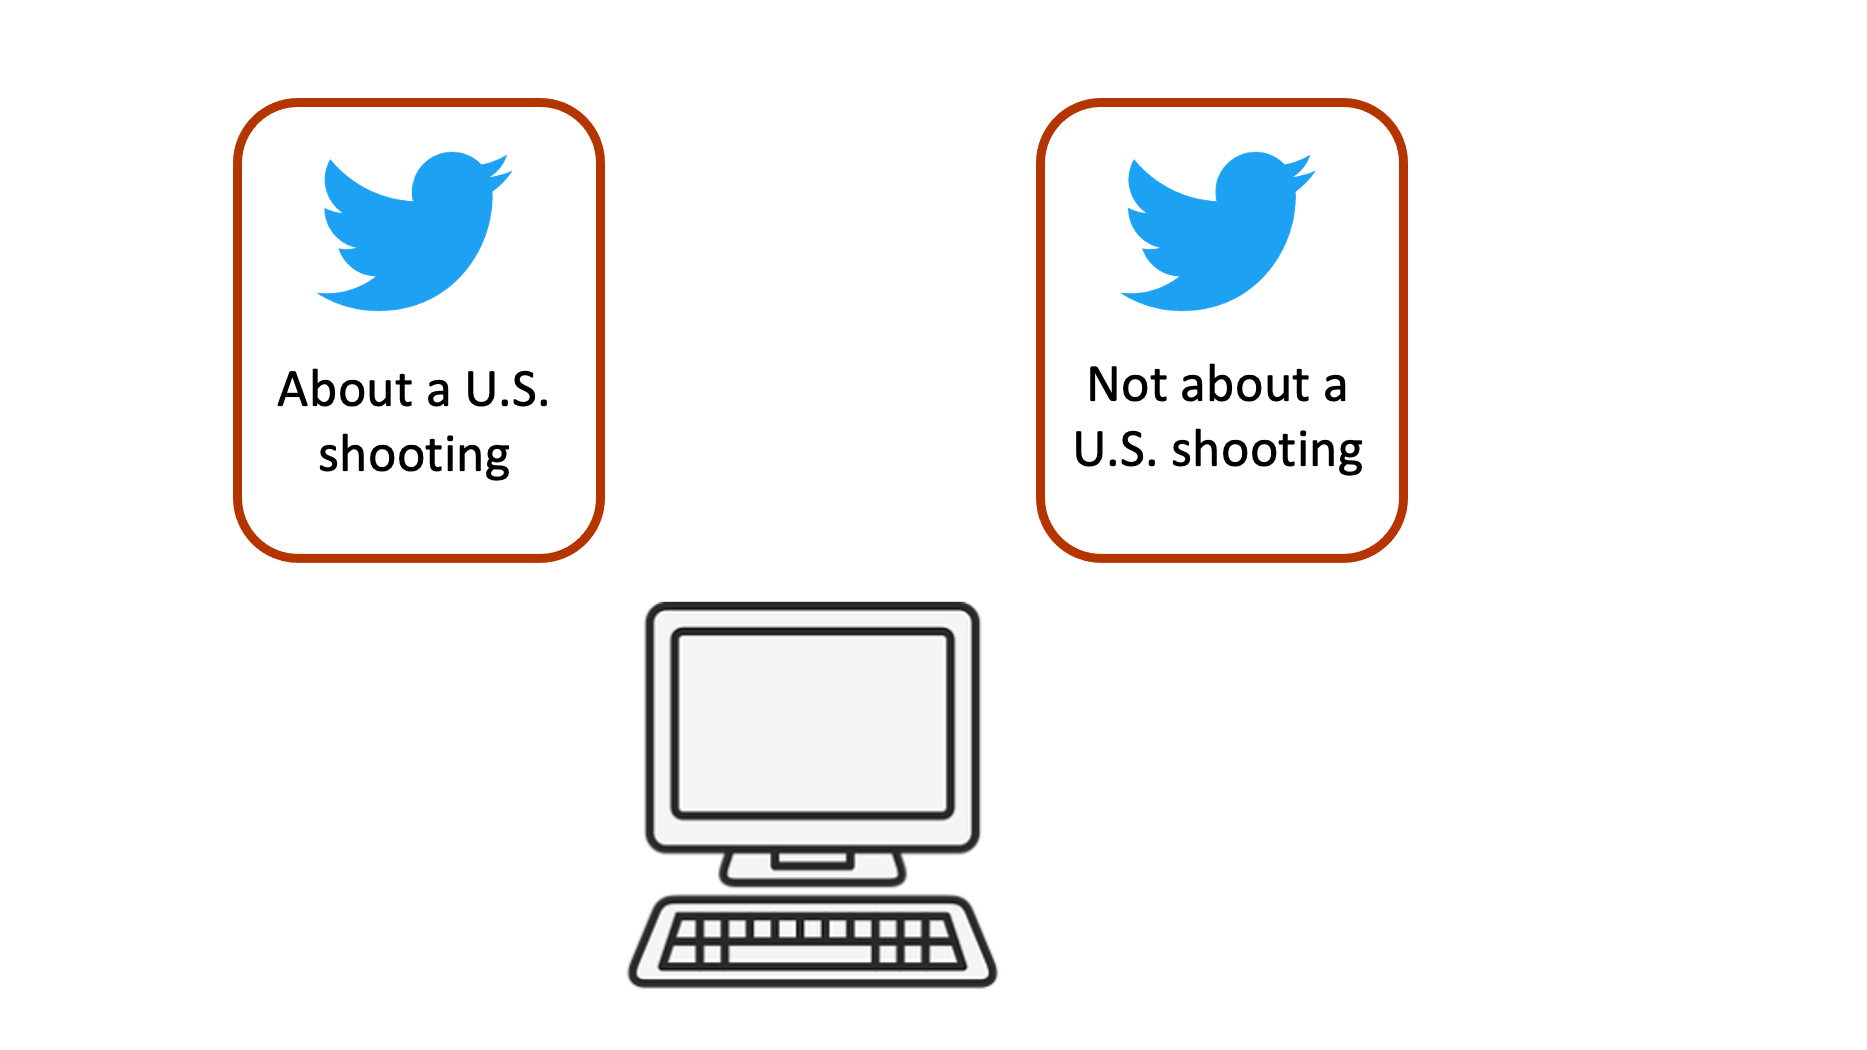
\includegraphics{../pictures/Zhangetal_1.png} \\\
	\end{center}
	
	\begin{tiny}
		\fullcite{zhang_whose_2019} 
	\end{tiny}
	
	% Using logistic regression in SML, it is possible to assign a category to millions of cases. How can this be used to study communication?
	
	% Example: Zhang et al. used it to analyze how people use Twitter to express grief after mass shootings. They trained a model to distinguish Tweets that were about U.S. shootings from Tweets that weren’t (two categories).
	
\end{frame}


\begin{frame}{Regression}
	
	\begin{center}
		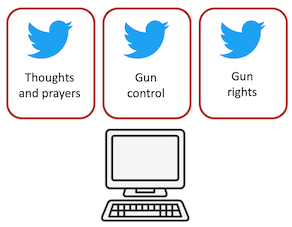
\includegraphics{../pictures/Zhangetal_2.png} \\\
	\end{center}
	
	\begin{tiny}
		\fullcite{zhang_whose_2019} 
	\end{tiny}
	
	% After that, they trained another model to classify relevant Tweets according to their topic in a more precise manner. Namely, the computer learned to indicate whether a Tweet was about “thoughts and prayers”, gun control or gun rights.
	
\end{frame}


\begin{frame}{Regression}
	
	\begin{center}
		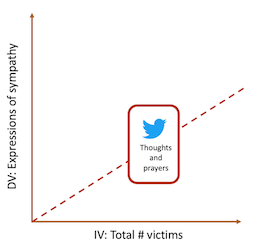
\includegraphics{../pictures/Zhangetal_3.png} \\\
	\end{center}
	
	\begin{tiny}
		\fullcite{zhang_whose_2019} 
	\end{tiny}
	
	
	% They then used these labels as the dependent variable in their analyses. The independent variables were (a) the total number of victims of a shooting and (b) the number of children killed. They found that mass shooting events involving both more total victims and more children killed generated more expressions of sympathy.
	
	% They also found that shootings with more African-America deaths or that are perpetrated by white shooters were related to fewer defenses of gun rights and calls for gun control…
	
\end{frame}


\begin{frame}[fragile]{What does this look like in code?}

First, we need to read in the ingredients we need for SML.
\begin{lstlisting}
import csv
from sklearn.model_selection import train_test_split

tweets = []
labels = []

with open(file) as fi:
     data = csv.reader(fi, delimiter='\t')
     for row in data:
          tweets.append(row[0])
          labels.append(row[1])

tweets_train, tweets_test, y_train, y_test = train_test_split(tweets, labels, test_size=0.2, random_state=42)
\end{lstlisting}
	
Where file is some file containg tweets (column 0) and their labels (column 1).
	
\end{frame}




\begin{frame}[fragile]{What does this look like in code?}
	
Second, vectorize the texts that need to be labeled: 

\begin{lstlisting}
from sklearn.feature_extraction.text import (TfidfVectorizer)

tfidfvectorizer = TfidfVectorizer(stop_words="english")
X_train = tfidfvectorizer.fit_transform(tweets_train)
X_test = tfidfvectorizer.transform(tweets_test)

\end{lstlisting}

Where tweets\_train and tweets\_test are two lists with tweets (strings)
	
\end{frame}


\begin{frame}[fragile]{What does this look like in code?}
	
Next, I train my machine and test it: 
	
\begin{lstlisting}
from sklearn.linear_model import (LogisticRegression)

logres = LogisticRegression()
logres.fit(X_train, labels_train)
y_pred = logres.predict(X_test)
\end{lstlisting}
	
\end{frame}


\begin{frame}[fragile]{What does this look like in code?}
	
To train a model based on a tf-idf vectorizer and Log Regression:
	
\begin{lstlisting}
from sklearn.feature_extraction.text import (TfidfVectorizer)
from sklearn.linear_model import (LogisticRegression)

tfidfvectorizer = TfidfVectorizer(stop_words="english")
X_train = tfidfvectorizer.fit_transform(tweets_train)
X_test = tfidfvectorizer.transform(tweets_test)

logres = LogisticRegression()
logres.fit(X_train, labels_train)
y_pred = logres.predict(X_test)
\end{lstlisting}
	
\end{frame}



\begin{frame}{Na\"{\i}ve Bayes}
	
	\begin{center}
		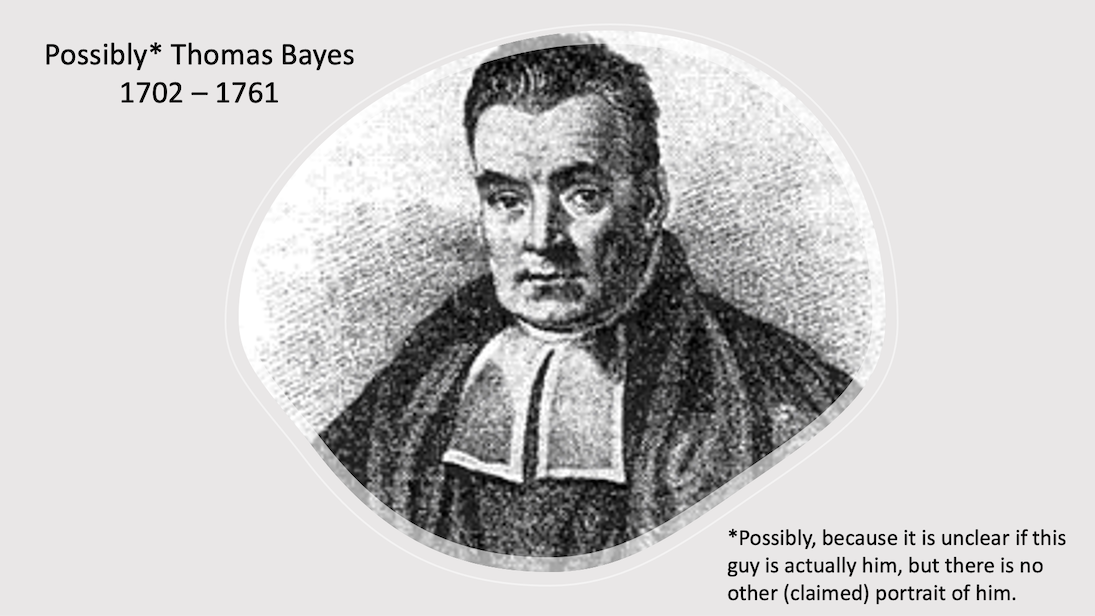
\includegraphics[width=\linewidth,height=\textheight,keepaspectratio]{../pictures/ThomasBayes.png} \\\
	\end{center}
	
	% Another way to predict a category is by using the Naïve Bayes classifier. Bayes because: It uses the theorem developed by Thomas Bayes. 
	
	% Naïve because: it assumes that all features are independent from each other. This is naïve because it is hardly ever the case. Think about survey data: one’s score on IV income is surely related to one’s score on IV education level. 
	
	% Although the assumptions of the Naïve Bayes classifier are often violated, it works remarkably well in practice. 
	
\end{frame}



\begin{frame}{Na\"{\i}ve Bayes}
	
	$ P(\rm{A} \mid \rm{B}) = \frac{P(\rm{B} \mid \rm{A}) \cdot P(\rm{A})}{P(\rm{B})} $
	
	Mathematicians’ language for: the probability of A if B is the case/present/true. 
	
	$ P(\rm{label} \mid \rm{features}) = \frac{P(\rm{features} \mid \rm{label}) \cdot P(\rm{label})}{P(\rm{features})} $
	
	
	% In our case it means: the probability of an item having a label, given a set of features. 
	
	% We use this formula to (1) train our model, (2) test it, and finally (3) evaluate our model.
	

\end{frame}


\begin{frame}[fragile]{What does this look like in code?}
	
Let's also train a model based on a count vectorizer and Naïve Bayes:
	
\begin{lstlisting}
from sklearn.feature_extraction.text import (CountVectorizer)
from sklearn.naive_bayes import MultinomialNBB

countvectorizer = CountVectorizer(stop_words="english")
X_train = countvectorizer.fit_transform(texts_train)
X_test = countvectorizer.transform(texts_test)

nb = MultinomialNB()
nb.fit(X_train, labels_train)
y_pred = nb.predict(X_test)
\end{lstlisting}
	
\end{frame}




\begin{frame}{Support Vector Machines}
	
	SVMs aim to find a hyperplane in an \(N\)-dimensional pace that distinctly classifies the datapoints.
	
	The best hyperplane is the one that has the maximum margin (distance) between the datapoints of both classes.
	
	\begin{center}
		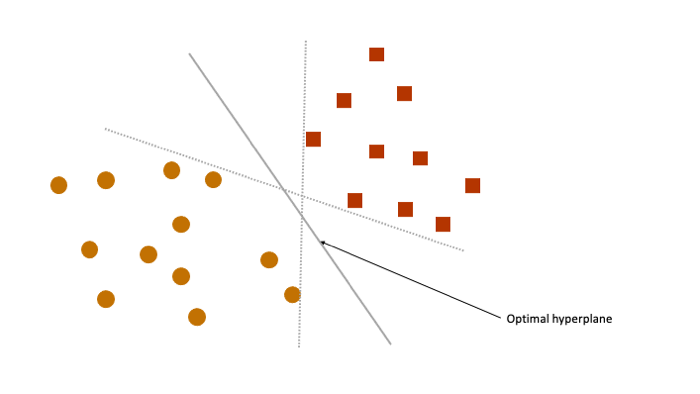
\includegraphics[width=\linewidth,height=0.5\textheight,keepaspectratio]{../pictures/optimal_hyperplane.png} \\\
	\end{center}
	
\end{frame}

\begin{frame}{Support Vector Machines}
	
	\begin{center}
		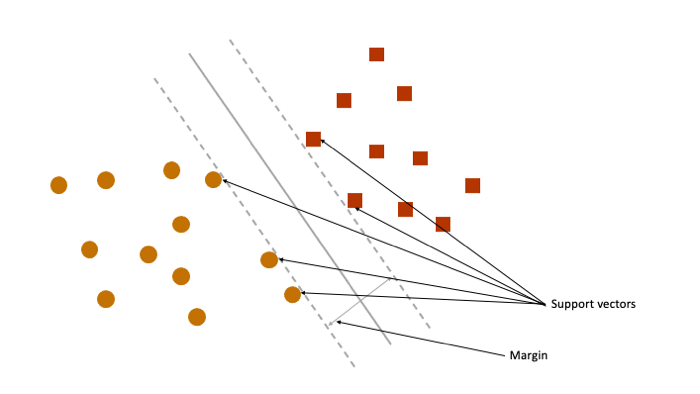
\includegraphics[width=\linewidth,height=\textheight,keepaspectratio]{../pictures/SVM.png} \\\
	\end{center}
	
\end{frame}


\begin{frame}{Decision Trees and Random Forests}
	
	\begin{center}
		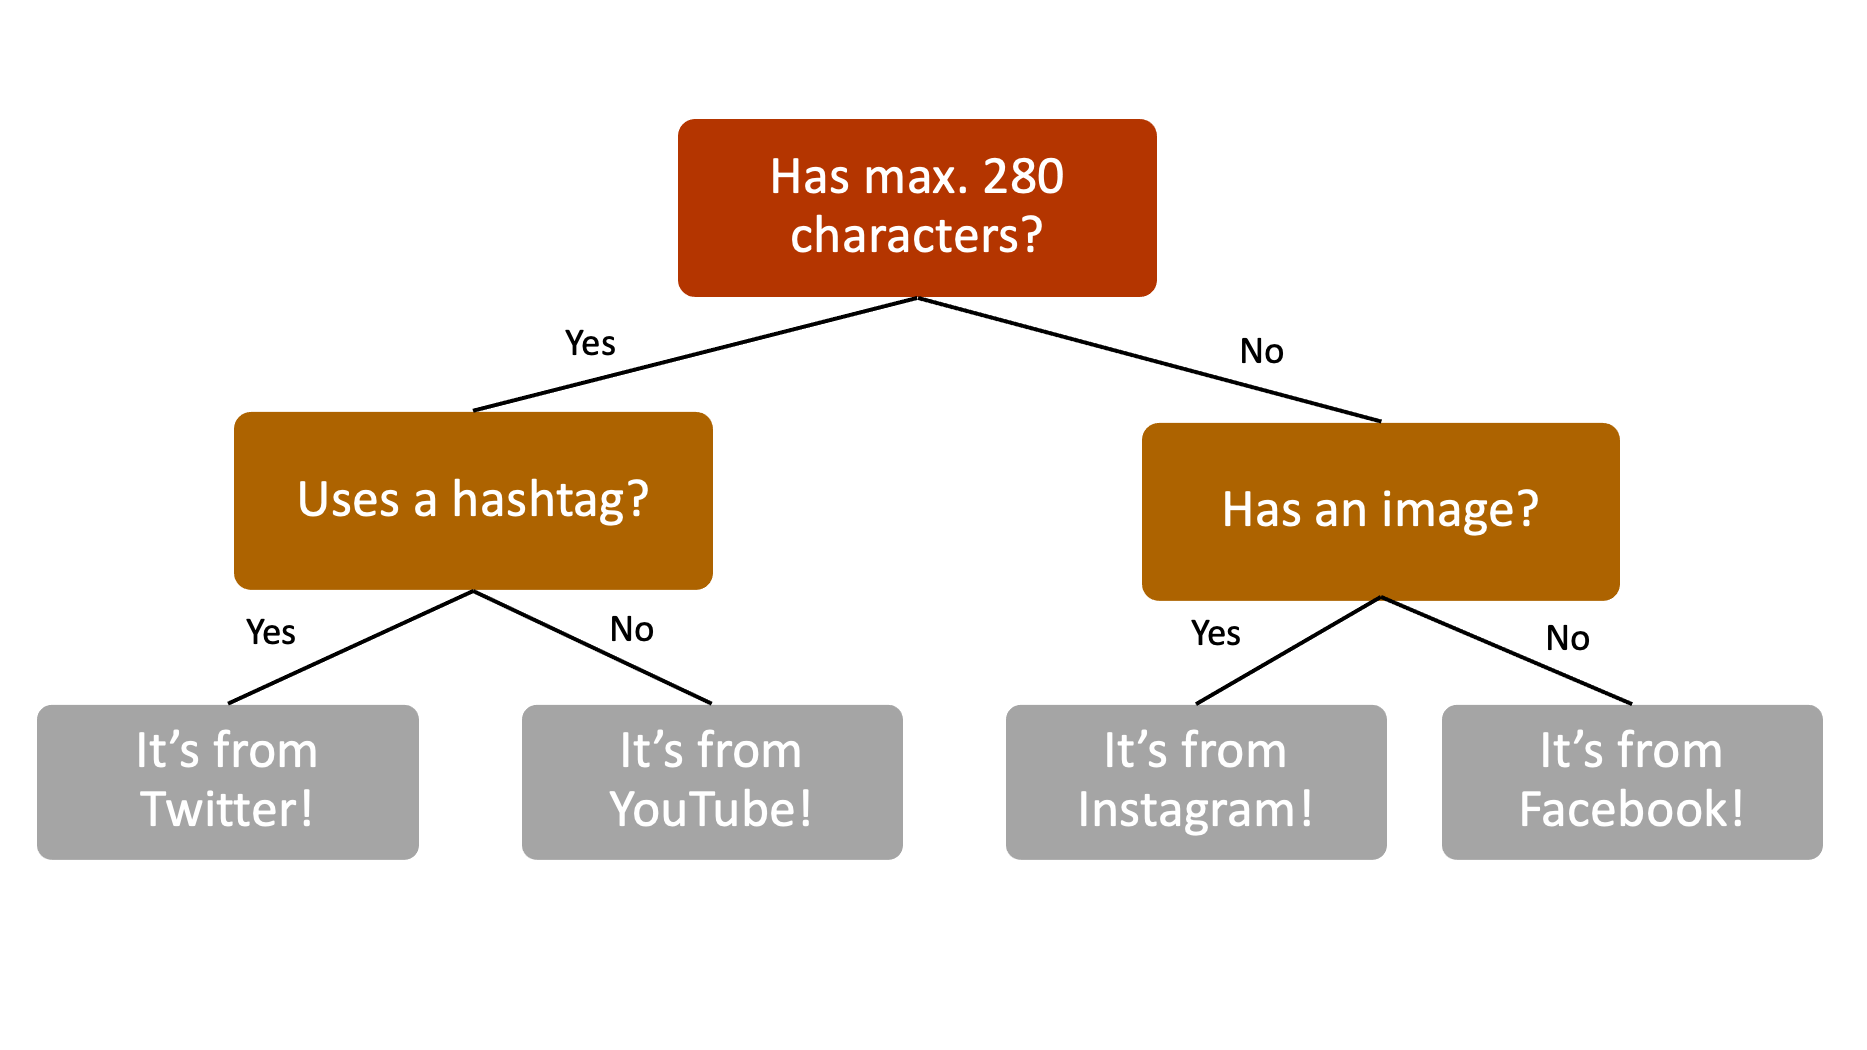
\includegraphics[width=\linewidth,height=\textheight,keepaspectratio]{../pictures/decisiontree.png} \\\
	\end{center}
	
	% In the previous sections, we discussed models that estimate linear relationships. So, we look at how an increase in an IV leads to a similar increase in the DV.
	
	% What about situations in which we want to know whether the value of a feature is above (or below) a specific threshold. For example, we want the computer to tell us the source of social media messages. 
	
	% Length is important here: If the message is longer than 280 characters, it cannot be from Twitter, for example. Note that this is the only thing we care about: whether a message is 281 characters long or 100.000 characters long doesn’t matter to us, we just want to know if it longer than 280 characters or not to be able to determine if Twitter is the source.
	
	% We can use a decision tree to learn more about this. This represents a stepwise decision process in which we first check one feature (i.e., the length) before checking another feature (e.g., presence of a hashtag).
	
	% Of course, this model will be wrong sometimes: some posts may be longer than 280 characters and contain an image but are posted on Facebook instead of Instagram, for example.
	
	% In Machine learning, the computer estimates this decision tree based on the data: it determines what features to look at and in what order to look at them.
	
	
\end{frame}



\begin{frame}{Decision Trees and Random Forests} 
	
	Advantages of decision trees:
	\begin{itemize}
		\item Transparency
		\item Suitable for non-linear relationships \\\
	\end{itemize}
	
	Disadvatanges of decision trees:
	\begin{itemize}
		\item Loss of nuance due to yes/no-design
		\item Cannot correct early mistakes
		\item Prone to overfitting
	\end{itemize}
	
	
\end{frame}


\begin{frame}{Decision Trees and Random Forests}
	
	\begin{center}
		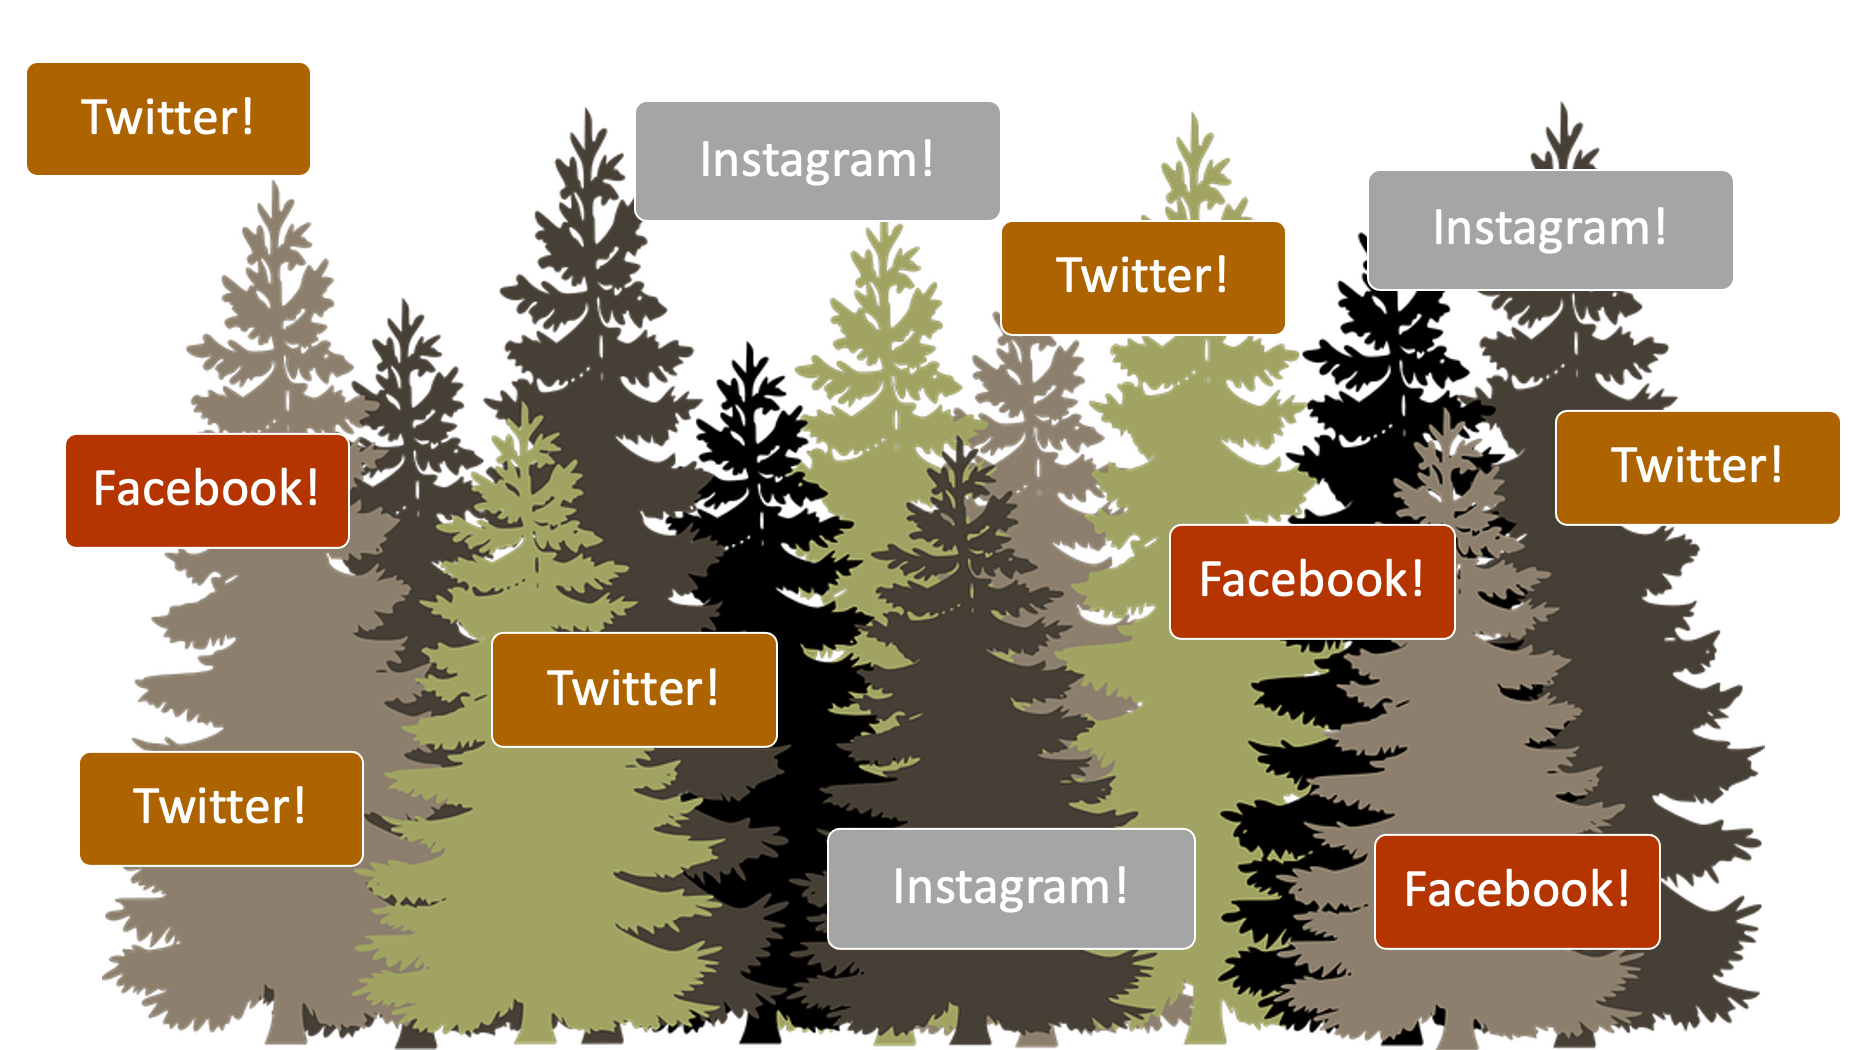
\includegraphics[width=\linewidth,height=\textheight,keepaspectratio]{../pictures/randomforest.png} \\\
	\end{center}
	
	% Solution to these disadvantages: Random forests! 
	
	% Drawing random samples from the data, multiple decision trees are estimated: we create a forest. We let each tree “vote” on what the outcome should be. This way, through majority voting, we come to a conclusion.
	
	% Using forests, we alleviate the problems of decision trees but we are still able to model non-linear relationships.
	
	% Connect to literature-example
	
\end{frame}




\begin{frame}{Recap}
	
	Many different models available for machine learning.
	
	How do you know what is the best for your case? Try it out and validate!
	
	% We discussed only a few of the many available models for machine learning. Which model is best, depends on the characteristics of your project. Often, researchers run multiple models and then evaluate them to determine which one works best for them.
\end{frame}



\begin{frame}{Zooming out} 
	
	We talked about:
	\begin{itemize}
		\item Rule-based Text Classification
		\item Automated Text Classification: SML
		\item The principles behind SML
		\item Some commonly used ML models \\\
	\end{itemize}
	
	Next, we will talk about:
	\begin{itemize}
		\item Validating models
	\end{itemize}
	
\end{frame}


\section{Validating models}


\begin{frame}{Precision and Recall}
	
	Precision quantifies the number of positive class predictions that actually belong to the positive cases. \\\ 
	OR: How much of what we found is actually correct?
	
	Recall quantifies the number of positive class prediction made out of all positive examples in the dataset. \\\
	OR: How many of the cases that we wanted to find did we actually find?
	
	% Comment:
	% Many different models that you can use! Which one is the best? Hard to say… often (as you could read for example, in Van Zoonen and Van der Meer for example) we try out different models and then we compare to determine which one is best. 
	
	% To validate models, we often use two measures: precision and recall.
	
	
\end{frame}



\begin{frame}{Precision and Recall}
	
	\begin{center}
		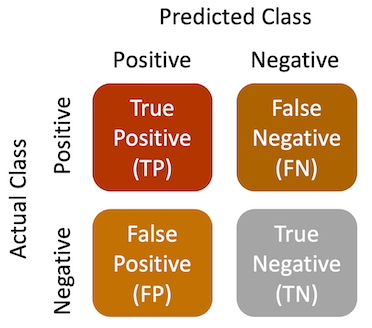
\includegraphics{../pictures/confusionmatrix_words.png} \\\
	\end{center}
	
	% To estimate precision and recall, we can create a confusion matrix.
	
	% This is a table where the columns represent the number of cases in a predicted class and the rows represent the number of cases in the real or actual class.
	
	% Imagine we build a sentiment classifier of movie reviews. We want to find only movies that received good reviews. So, we have two goals: we want to receive as many good movies as possible (recall) and we also want to find only good movies (and not movies that got many bad reviews) (precision).
	
	
\end{frame}


\begin{frame}{Precision and Recall} 
	
	\begin{columns}
		\column{.3\textwidth}
		\makebox[\columnwidth]{
			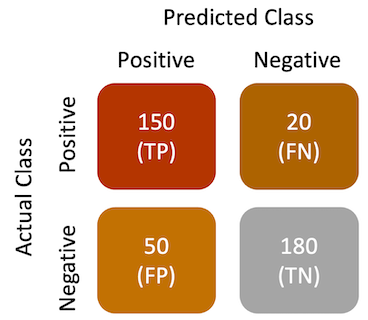
\includegraphics[width=\columnwidth,height=\paperheight,keepaspectratio]{../pictures/confusionmatrix_numbers.png}}
		\column{.7\textwidth}
		Precision is calculated as: \(\frac{\rm{TP}}{\rm{TP}+\rm{FP}}\) \\\
		In our case \(\frac{\rm{150}}{\rm{150}+\rm{50}}\) which is \(0.75\) \\\
		Recall is calculated as \(\frac{\rm{TP}}{\rm{TP}+\rm{FN}}\) \\\
		In our case \(\frac{\rm{150}}{\rm{150}+\rm{20}}\) which is \(0.88\)
	\end{columns}
	
	
	% A not precise model may find a lot of the positives, but its selection method is noisy: it also wrongly detects many positives that aren’t actually positives.
	% A precise model is very “pure”: maybe it does not find all the positives, but the ones that the model does class as positive are very likely to be correct
	
	% A model with high recall succeeds well in finding all the positive cases in the data, even though they may also wrongly identify some negative cases as positive cases.
	% A model with low recall is not able to find all (or a large part) of the positive cases in the data.
	
\end{frame}


\begin{frame}[fragile]{What does this look like in code?}
	
Let's ask for a confusion matrix: 

\begin{lstlisting}
from sklearn.metrics import confusion_matrix

y_test = [0, 1, 1, 1, 0]
y_pred = [0, 0, 1, 1, 1]

print(confusion_matrix(y_test, y_pred))
\end{lstlisting}

\begin{lstlistingoutput}
[[1  1 ]
[ 1  2]]
\end{lstlistingoutput}
	
\end{frame}


\begin{frame}[fragile]{What does this look like in code?}
	
Let's get some metrics for validation: 
	
\begin{lstlisting}
from sklearn.metrics import classification_report
print(classification_report(y_test, y_pred))
\end{lstlisting}
	
\begin{lstlistingoutput}
              precision    recall  f1-score   support

0       0.50      0.50      0.50         2
1       0.67      0.67      0.67         3

accuracy                           0.60         5
macro avg       0.58      0.58      0.58         5
weighted avg       0.60      0.60      0.60         5
\end{lstlistingoutput}
	
\end{frame}


\begin{frame}{\(F_1\)-score}
	
	\(F_1\)-score: The harmonic mean of precision and recall. \\
	
	\(F_1\)-score \(= 2 \cdot \frac{\rm precision \cdot recall}{\rm precision + recall}\)
	
	% Since the F1 score is an average of Precision and Recall, it means that the F1 score gives equal weight to Precision and Recall:
	% A model will obtain a high F1 score if both Precision and Recall are high
	% A model will obtain a low F1 score if both Precision and Recall are low
	% A model will obtain a medium F1 score if one of Precision and Recall is low and the other is high
	
	
\end{frame}



\begin{frame}{Precision and Recall}
	
	\begin{center}
		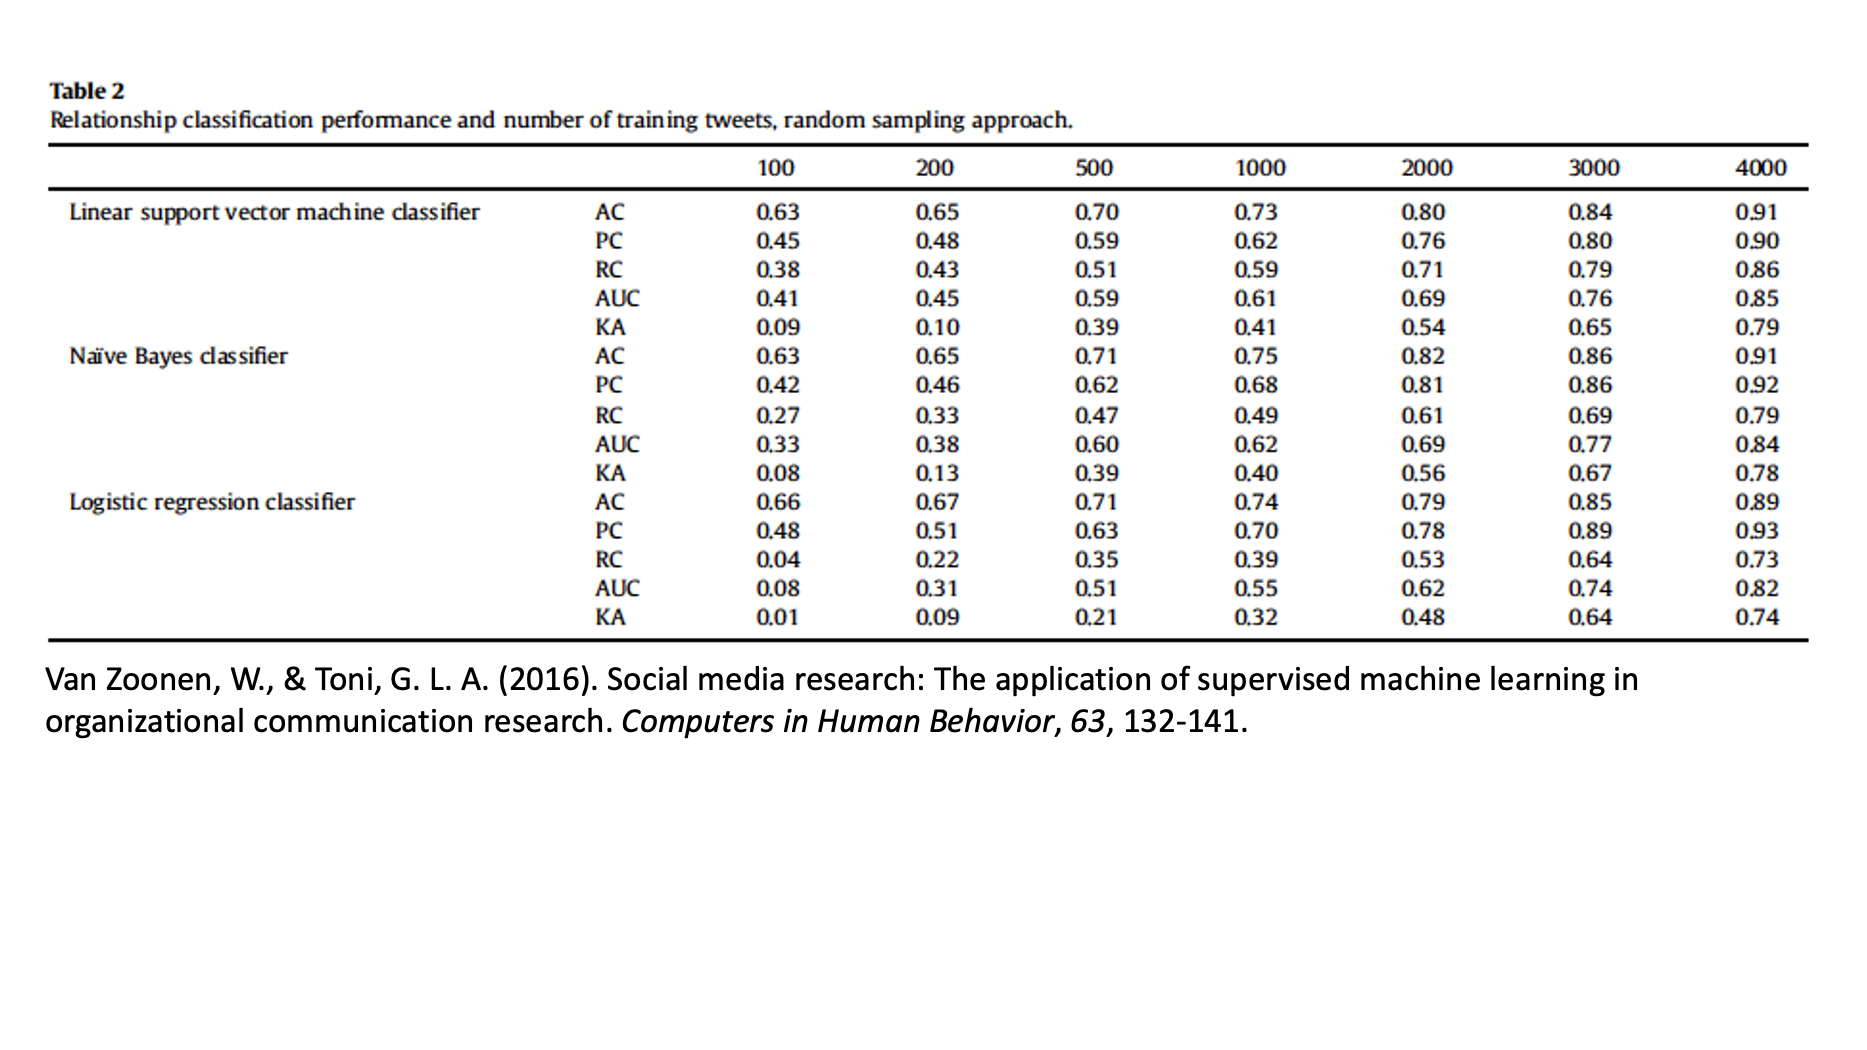
\includegraphics[width=\linewidth,height=\textheight,keepaspectratio]{../pictures/VanZoonen.png} \\\
	\end{center}
	
	\begin{tiny}
		\fullcite{van_zoonen_social_2016} 
	\end{tiny}
	
	
	% Discuss example: Van Zoonen & Van der Meer (2016)
	
	% As you read in this paper, there are more metrics in addition to precision and recall. 
	
\end{frame}






\begin{frame}{Accuracy}
	
	Accuracy: In which percentage of all cases was our classifier right? \\
	
	Class distribution: The number of examples that belong to each class. \\
	
	Imbalanced classification: A classification predictive modeling problem where the distribution of examples across the classes within a training dataset is not equal.
	
	% Slide about accuracy. Discuss class imbalance (https://machinelearningmastery.com/what-is-imbalanced-classification/)
	
\end{frame}


\begin{frame}{Accuracy}
	
	\begin{center}
		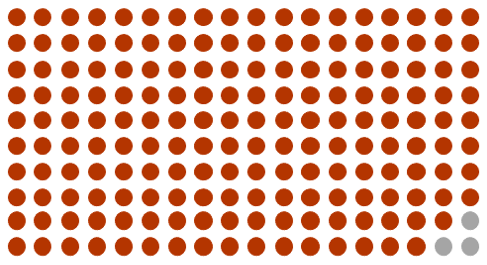
\includegraphics[width=\linewidth,height=\textheight,keepaspectratio]{../pictures/imbalance.png} 
	\end{center}	
	
	Majority class (red dots) vs. minority class (grey dots) 
	
	% Problem of imbalance remains to be solved
	% Some examples in which this is a problem: fraud detection, spam detection... and outlier detection
	
	%Linking back to accurcay: if we would label all dots as "red", we get a high accuracy score: we were right in almost all cases. But how valuable is this: we missed those crucial three cases that we wanted to learn more about!
	
	%More: https://machinelearningmastery.com/what-is-imbalanced-classification/	
\end{frame}



\begin{frame}{Validating Models}
	
	Many more metrics to validate models. \\
	
	Learn more using, for example, the scikit-learn documentation. 
	
\end{frame}



\begin{frame}{Zooming out} 
	
Today, we talked about:
\begin{itemize}
	\item Rule-based Text Classification
	\item Automated Text Classification: SML
	\item The principles behind SML
	\item The steps of SML
	\item Some commonly used ML models
	\item Validating models \\\
\end{itemize}

In this week's tutorial, you will:
\begin{itemize}
	\item Present your group projects
\end{itemize}
	
\end{frame}


\begin{frame}
	
To do before next lecture:
	\begin{itemize}
		\item Make the homework assignments for week 8: Complete the first five questions of next week's tutorial exercises (available on Github)
	\end{itemize}
	
\end{frame}



	
\end{document}